\documentclass{ximera}

\begin{document}

\begin{question}
  Find 
  \[
  \displaystyle \lim_{x\to 0} f(x)
  \]
  where
  \[
  f(x) = \left\{\begin{array}{cl} \cos x & x\leq 0, \\ x^2+3x+1 & x>0. \end{array}\right.
  \]
  \begin{solution}
    \begin{hint}
     Both $\cos x$, for $x\leq0$, and $x^2+3x+1$, for $x>0$ are continuous on their respective domains. However, for the limit $\lim\limits_{x\to0}f(x)$ to exist, both the left-hand and the right-hand limits must exist and be equal.
    \end{hint}
     \begin{hint}
    	Take a look at the graph of the function
    \begin{center}
     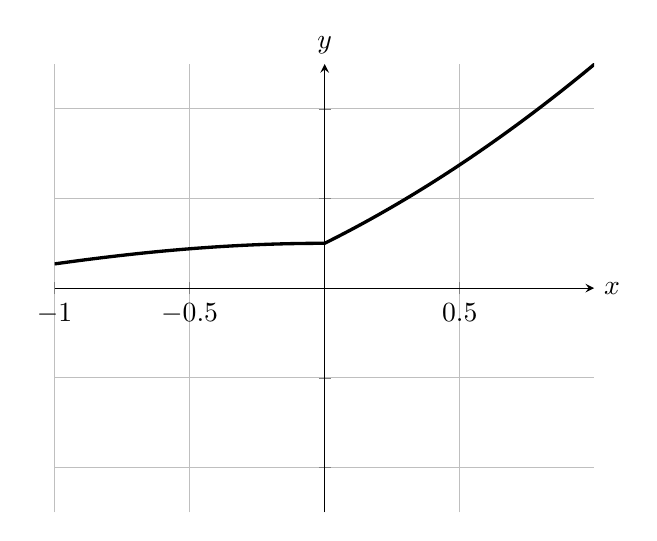
\begin{tikzpicture}
	\begin{axis}
	[ymin=-5,ymax=5, axis lines=center,xlabel=$x$,ylabel=$y$,every axis y 
	label/.style={at=(current axis.above origin),anchor=south},every axis x label/.style={at=(current axis.right of origin),anchor=west},
	domain=-2:2,
	yticklabels={},
	ymajorgrids=true,
	grid = major
	]
	\addplot[domain=-1:1,very thick,smooth,samples=1000]
	{(!(\x>0))*(cos(deg(\x)))+(\x>0)*(\x^2+3*\x+1)};
	\end{axis}
       \end{tikzpicture}      
      \end{center} 
    \end{hint}
    \begin{hint}
     Evaluating $\lim\limits_{x\to0^{+}}f(x)$ we see that it tends to $1$. This follows because, for $x>0$, we are on the piece of $f(x)$ given by $x^2+3x+1$ and the limit $\lim\limits_{x\to0}x^2+3x+1=1$, certainly. On the other hand, evaluating $\lim\limits_{x\to0^{-}}f(x)$ we see it tends to $1$. This follows because, for $x\leq0$, we are on the piece of $f(x)$ given by $\cos x$ and the limit $\lim\limits_{x\to0}\cos x=1$, certainly. These are equal.
    \end{hint}
     The limit, $\lim\limits_{x\to0}f(x)=$
    \answer{$1$}.
  \end{solution}
\end{question}

\end{document}